\documentclass[11pt,letter]{article}
\usepackage[top=1.00in, bottom=1.0in, left=1.1in, right=1.1in]{geometry}
\usepackage{graphicx} % Required for inserting images
\usepackage{xcolor} 
\definecolor{Accent}{HTML}{bd2b00} 
\usepackage{natbib}
\usepackage{hyperref}
\hypersetup{colorlinks,citecolor = Accent, linkcolor = Accent,urlcolor = Accent, breaklinks=true}
\usepackage{cleveref}
\usepackage[labelfont=bf]{caption}
\bibliographystyle{amnat}


\title{Solstice optimizes thermal growing season}

\author{Victor, Lizzie}
\date{Aug.-Nov. 2024}

\begin{document}

\maketitle

%\begin{enumerate}

%\item New (recent) exciting findings! Solstice, "\emph{celestial starting gun}"\\
%(Bad) consequences for climate change forecasting: plants are stuck? \\
% $\rightarrow$ But leave an open question: why solstice?
Plants generally use environmental cues, such as temperature and photoperiod, to adjust the timing of phenological events in response to environment variability within and between years. Yet, the larger mechanisms behind these cues remain largely unknown for many events, leaving a critical gap in our understanding of how plants will respond and adapt to future climates.
% Gao2024: "we do not know when plants start responding to temperatures, what range of temperatures influences spring phenology, and how and why these controls vary by species or climate conditions"

Recently, summer solstice has been proposed as a universal trigger to modulate cues and initiate key physiological processes \citep{Zohner2023, Journe2024}---an idea that builds on earlier suggestions of solstice-driven control of tree growth \citep{Rossi2006}. This proposed photoperiod switch, if correct, could reshape predictions of forest responses to climate change. 
However, using a fixed date like the solstice as a cue could limit plasticity and become less suitable in a warmer future climate \citep{Wolkovich2021}. 
This may in turn drive forest declines, with significant implications for carbon storage, and thus raises important questions about the suitability for plants to rely on the solstice. 

% \item Plants need to balance transition to events at best moment vs end-of-season constraint, i.e. choose when to transition without full info\\
% $\rightarrow$ Need to optimize predictions!
The timing of major plant phenological transitions---such as start of growth with leafout---should match development states with fitness opportunities, given no other constraints. In most environments, this will always involve a trade-off between an increased fitness (e.g. a longer window for growth) and an increased susceptibility to climatic and biotic risks (e.g. a higher exposition to late frosts). Because plants cannot know these exact opportunities and risks in advance, they should rely on the most informative cues to accurately anticipate environmental conditions and optimize their chances for growth and reproduction \citep{Chevin2015, Bonamour2019}.

% \item (Thermal) $GDD$ as a critical integrator\\
% Critical both to crops and wild plants\\
%Plants want to grow as much as possible during warm years, and benefit from warm years to set many flowers (flower differentiation?)
In particular, it is well established that plants respond primarily to integrated climate forcing \citep{Chuine2017}, often measured as the accumulation of temperatures, in a given range---where metabolism is sufficient---and over a given period (growing degree-days, GDD). This heat accumulation is a key factor in development and growth processes of both crops \citep[e.g.][]{Cross1972} and wild plants \citep[e.g.][]{Hunter1992}. The number of GDD accumulated throughout the season directly impacts how quickly cells elongate to form new organs and how quickly a plant progresses through growth stages. Plants are thus expected to take full advantage of warmer years (with a high GDD accumulation) to maximize growth and set many flowers for the following season.

% \item Given $GDD$ is so important, plants should thus transition into events when they can best predict $GDD_{total}$ within growing season -- while still having enough time/energy \emph{to do what they need to do}
Given the importance of GDD, plants should ideally time their transitions when their ability to predict the total GDD within the growing season is maximum while still having enough potential thermal energy to complete essential growth and reproductive processes. Concretely, this trade-off means that there should be an optimal period during which the plant has accumulated enough GDD to reliably predict the total GDD by the end of the year (\emph{environmental predictability}), while also maximizing the remaining GDD available (\emph{growth potential}). Here, we define the environmental predictability at a day $d$ as the $R^2$ of a linear regression, across years, between the total GDD (that will be accumulated at the end of the year) and the GDD already accumulated between 1st January and $d$ (supp Fig). 
This simple definition allows us to examine which window in the season appears optimal for the plant to maximize its growth and development while minimizing risks.

\begin{figure}[h]
\centering
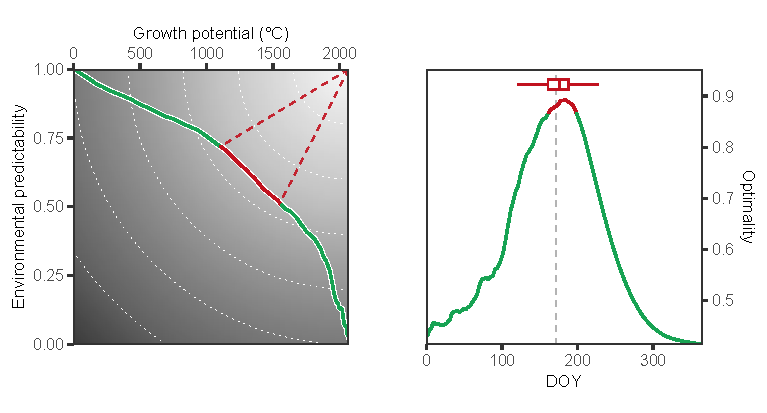
\includegraphics{global_optimality.pdf}
\vspace*{-0.7cm}
\caption{\textbf{Solstice marks the optimal trade-off between environmental predictability and growth potential.}}
\label{fig:globaloptimality}
\end{figure}

% \item We found this optimal point in Europe to be the solstice(ish)\\
% \begin{enumerate}
%     \item If this true widely, then evolution towards an universal solstice trigger could make sense, right? 
%     \item But our results also suggest we cannot teasee appart solstice and thermal optimum-predictability cue
% \end{enumerate}
Globally, we found the optimal period to be around the summer solstice in Europe (\Cref{fig:globaloptimality}). Solstice appears as a critical juncture for the optimization of both environmental predictability and growth potential.
If this specific day indeed represents a broad-scale optimum across different climatic conditions, genetic evolution towards a universal solstice trigger could make sense---especially since this optimum was stable over the Holocene (supp Fig). 
It could act as a reliable "marker" for when a plant has likely accumulated the right amount of GDD.
Yet, our results also suggest it is challenging to disentangle the influence of the solstice from that of a thermal optimum cue.
% does solstice coincide with the period of highest thermal energy in temperate regions? Peak of daily GDD is rather after solstice...
This could indicate that plants rely on a combination of both solstice and thermal cues to optimize growth and reproductive timing. 
Alternatively, this overlap could simply be a coincidence, since it would be costly for plants to closely track two different signals---i.e. to encode and decode both thermal and photoperiod information within their cells. 


% \item Supporting this we found important variation over space (and time?)
Supporting this "cautionary" hypothesis, our results reveal substantial variation in the optimal timing across Europe (\Cref{fig:localoptimality}). In warmer southern Europe, plants reach an optimum earlier in the season, whereas in northern regions, cooler temperatures delay this timing beyond the solstice. 
This regional variability suggests that plants should likely be partially adapted to their local climates---and especially to how GDD accumulate in their specific environment.
From a parsimonious perspective, tracking primarily GDD might be more straightforward and aligned directly with the actual energy a plant needs to grow and reproduce. % (= directly linked to metabolic processes)
Tracking the solstice is likely more complex. Indeed, plants would need to sense not just the day length but also the variation in the rate of change of day length over time---essentially, the second derivative.
% more directly beneficial for the plant?
% What would be the benefit to have a separate mechanism, with the risk of a potential redundancy of tracking both the solstice and thermal cues? (but which thermal cue to track the optimal period?)

% Maybe we need to talk more about photoperiod cue sensing? What is known ("not a new result" Isabelle...) => make a paragraph?
% second derivative sensing seems unlikely, but we know photoperiod can be important?
% what could be the benefit of tracking photoperiod => synchronize populations broadly?
% if plants don't use solstice or if they don't use photoperiod, which cue(s) they need to track to understand that it is the optimal period, ? Temperature (and daily GDD accumulation) peaks after the optimum, so it should be something else?
% Does using solstice will prevent adaptative plasticity in future climate, ie plants could be "locked in a solstice response" (and mention supp figure with CMIP6 projections?)
% + "photosynthetic capacity peaks just after summer solstice and declines with decreasing photoperiod, before air temperatures peak" https://www.pnas.org/doi/10.1073/pnas.1119131109#fig02


% \begin{enumerate}
%     \item critical need for experiments to disentangle daylength vs temp.
%     \item researchers need to more clearly test for (i) trends estimated at local scale across gradient and (ii) how they scale up to (sub)continental/global scales
% \end{enumerate}
Disentangling the role of the solstice as a cue for plant phenology is challenging, as plants have already started accumulating GDD several months before the solstice.
Complex natural correlations in environmental data may generate spurious results \citep{Gao2024}. % "inherent correlations in climate in regions that the field does not fully understand/incorporate"
To address this, there is a critical need for carefully designed experiments that control for the covariation between temperature and photoperiod  \citep{Buonaiuto2023}.
Beyond controlled experiments, researchers must also better examine local-scale trends and how they scale up to subcontinental scales. Understanding how plant responses to photoperiod and temperature vary regionally will help clarify broader synchrony patterns.
% =>  and finally: inform phenological models, allowing researchers to build more accurate predictions by incorporating the specific cues plants use to trigger growth

\begin{figure}[h]
\centering
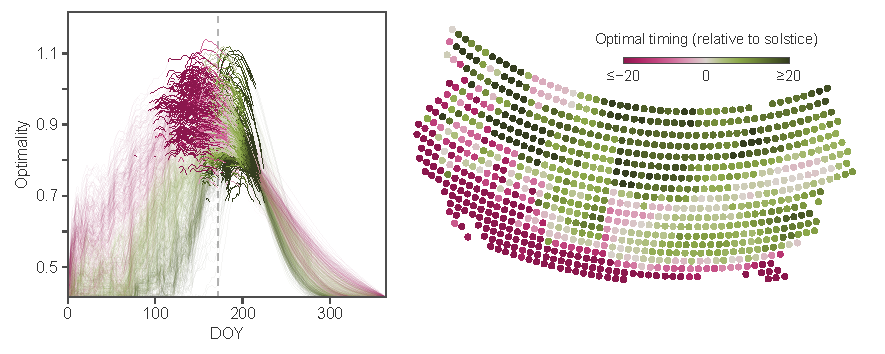
\includegraphics{local_optimality.pdf}
\vspace*{-0.7cm}
\caption{\textbf{Variation in optimal timing reflects different climatic conditions across Europe.}}
\label{fig:localoptimality}
\end{figure}

%\end{enumerate}

\bibliography{synchrony}

\end{document}
